% По умолчанию используется шрифт 14 размера. Если нужен 12-й шрифт, уберите опцию [14pt]
%\documentclass[14pt]{matmex-diploma}
\documentclass[14pt]{matmex-diploma-custom}

\begin{document}
% Год, город, название университета и факультета предопределены,
% но можно и поменять.
% Если англоязычная титульная страница не нужна, то ее можно просто удалить.
\filltitle{ru}{
    chair              = {Программная инженерия\\Системное программирование},
    title              = {Универсальный механизм первичного поиска повторов в тексте для пакета Duplicate Finder},
    % Здесь указывается тип работы. Возможные значения:
    %   coursework - Курсовая работа
    %   diploma - Диплом специалиста
    %   master - Диплом магистра
    %   bachelor - Диплом бакалавра
    type               = {master},
    position           = {студента},
    group              = 21.М07-мм,
    author             = {Глазырин Антон Георгиевич},
    supervisorPosition = {доц. каф. СП, к.ф.-м.н.},
    supervisor         = {Луцив Д.\,В.},
    reviewerPosition   = {ген. дир. ООО <<Ембокс>>},
    reviewer           = {Бондарев А.\,В.},
%   university         = {Санкт-Петербургский Государственный Университет},
%   faculty            = {Математико-механический факультет},
%   city               = {Санкт-Петербург},
%   year               = {2013}
}

\filltitle{en}{
	chair              = {Software and Administration of Information Systems \\ Software Engineering},
	title              = {Universal initial duplicate search engine for the Duplicate Finder toolkit},
	% Здесь указывается тип работы. Возможные значения:
	%   coursework - Курсовая работа
	%   diploma - Диплом специалиста
	%   master - Диплом магистра
	%   bachelor - Диплом бакалавра
	type               = {master},
	author             = {Anton Glazyrin},
	supervisorPosition = {C.Sc., Associate Professor},
	supervisor         = {Dmitry Luciv},
	reviewerPosition   = {CEO of "Embox" co.ltd.},
	reviewer           = {Anton Bondarev},
	%   university         = {Санкт-Петербургский Государственный Университет},
	%   faculty            = {Математико-механический факультет},
	%   city               = {Санкт-Петербург},
	%   year               = {2013}
}

\maketitle
\tableofcontents
\setcounter{secnumdepth}{4}

%==============================================================================
% У введения нет номера главы
\section*{Введение}
Документация является неотъемлемой частью большинства крупных проектов. При этом с ростом и развитием продукта она становится все объемнее и запутаннее: на первых этапах жизненного цикла проекта документация может отсутствовать совсем, однако чем дольше проект находится в фазе реализации, тем больше функционала и особенностей нужно документировать. Неудивительно, что со временем на поддержку документации будет тратится все больше сил и времени, что затрудняет сопровождение проекта.

В целом документацию можно разделить на два типа: описательную и справочную \cite{bib:art:DocumTypes}. Описательная документация нужна для общего ознакомления пользователя с продуктом: она не содержит много деталей работы продукта или технических подробностей, и в основном представлена естественным языком. Справочная, наоборот, ориентирована на пользователей, которые уже разбираются в предметной области, и просто хотят найти какую-либо специфичную информацию. Поэтому, справочная документация обычно является сводкой существующего функционала: список методов, интерфейсов и т.п., и часто представлена исходным кодом. На практике, в одном документе могут быть фрагменты обоих типов, то есть документация является сочетанием естественного языка и исходного кода.

Одним из наиболее влиятельных факторов усложнения ведения документации является наличие большого количества повторов. Они не только могут сильно раздувать общий объем, но также из-за них усложняется сохранение целостности --- одно и то же изменения приходится вносить несколько раз в разные части документации, что легко может привести к ошибкам и пропускам. Исследования также показывают, что повторы могут существовать практически в любом документе, и их наличие не зависит от конкретики продукта \cite{bib:art:JuergensCloneDetect, bib:art:DuplicatesStudy}. Кроме того, в этих работах подтверждается, что повторы действительно оказывают негативное влияние на общее качество документации.

Сам по себе поиск повторов практически всегда является некоторой подзадачей для достижения более осмысленной цели, поэтому он применяется в совершенно различных областях \cite{bib:art:NearDupSurvey}. Например, в сфере разработки ПО наибольшее внимание уделяется поиску клонов в исходном коде \cite{bib:art:SoftwareClonesSurvey}. Инструменты, основанные на этом подходе, предоставляют широкий спектр возможностей, от помощи с рефакторингом, до анализа недостатков глобальной архитектуры.

Однако, что касается более частной задачи поиска повторов в документации, данной теме уделяется не слишком много внимания, а если она и затрагивается, то лишь поверхностно. Существующие инструменты для работы с исходным кодом полагаются на достаточно специфичные особенности, такие как жесткая структура программы, семантика языков и т.п. \cite{bib:tool:ASTSearch, bib:tool:ASTRefactor, bib:tool:ASTSuffix}. Такие методы плохо подходят для работы с документацией из-за того, что она содержит не только фрагменты исходного кода, но и фрагменты на естественном языке.

Для решения задачи поиска повторов в документации был создан исследовательский прототип --- Dupilcate Finder Toolkit \cite{bib:tool:DuplicateFinder}, основной целью которого является работа с документацией. Данный инструмент представляет собой университетскую разработку, которая делалась многими людьми на протяжении большого временного промежутка, из-за чего проект состоит из множества составных частей, что сильно усложняет поддержку и дальнейшее развитие.

Особенно стоит отметить проблемы с компонентами, непосредственно отвечающими за поиск повторов \cite{bib:tool:CloneMiner, bib:tool:FuzzySearch, bib:tool:ImprovedNgramSearch}: они написаны на разных языках, некоторые из них являются внешними закрытыми разработками, они не разделяют потоков данных, повторяют некоторые этапы анализа несколько раз и в целом работают изолированно друг от друга. Для улучшения работы с пакетом было бы разумно разработать единую компоненту, целиком реализующую весь необходимый функционал.

%==============================================================================
\section{Постановка задачи}
Целью данной работы является разработка и реализация унифицированной подсистемы поиска точных и неточных повторов для Duplicate Finder Toolkit и ее интеграция с заменой существующих компонент. Для достижения этой цели в рамках работы были сформулированы следующие задачи.

\begin{enumerate}
	\item Анализ предметной области --- поиск повторов в текстах различных видов.
	\item Определение проблем поиска повторов в DuplicateFinder и требований к новому механизму.
	\item Проектирование конвейера механизма поиска повторов.
	\item Разработка алгоритмов точного и неточного поиска.
	\item Реализация инструмента и его интеграция в DuplicateFinder.
	\item Проведение тестирования разработанного инструмента.
\end{enumerate}

%==============================================================================
\section{Обзор предметной области}
\subsection{Поиск повтров в различных сферах}
Поиск повторов применяется во многих областях для достижения разнообразных целей \cite{bib:art:NearDupSurvey}. При этом непосредственно сам поиск практически никогда не является конечной целью. Найденные повторы могут быть использованы, например, как входные данные для различных инструментов, или для проведения некоторого анализа. Благодаря тому, что задача поиска повторов является достаточно самостоятельной и обособленной, существует множество инструментов для ее решения, часто заточенных под свою конкретную область применения.

Неточное сравнение широко распространено в задачах, где необходимо вычислять схожесть текстов. Например, поиск неточных повторов лежит в основе большинства инструментов проверки на плагиат. В работе \cite{bib:tool:Allign} рассматривается метод вычисления схожести двух документов путем сравнения текстовых фрагментов. Для сравнения используется подход min-hash \cite{bib:art:MinHash}. Авторы инструмента \cite{bib:tool:TxtAling} продолжили эту тему в своей работе. Вместо непосредственного сравнения фрагментов они предложили группировать их при помощи подхода bottom-k sketches \cite{bib:art:Bottom-sketch}. Данный метод позволяет не только определять схожие фрагменты в двух документах, но и оптимально выбирать документ, с которым будет производиться сравнение. Еще одним распространенным подходом, основанном на хешировании, является sim-hash \cite{bib:art:SimHash}. Он позволяет получить <<отпечатки>> (fingerprints) текстов и использовать их для быстрого вычисления приблизительной оценки схожести. Такой метод помогает оптимизировать обработку больших объемов данных, как, например, показано в работе \cite{bib:tool:SpamDetect}.

Достаточно широко распространены средства для поиска повторов в программном коде, так как обнаружение дублированных участков кода помогает избежать ряда проблем и открывает возможности для улучшения системы \cite{bib:art:SoftwareClonesSurvey, bib:art:SoftwareClonesReview}. Кроме того, наличие большого количество работ по этой теме можно объяснить и тем, что согласно исследованиям \cite{bib:art:LagueCloneStudy, bib:art:BakerCloneStudy} около 5--10\% кода в больших проектах является дублированным, что составляет достаточно значительную часть. Одним из основных подходов для обнаружения дубликатов является анализ синтаксического дерева программы. Такие инструменты как \cite{bib:tool:ASTRefactor, bib:tool:ASTSearch} позволяют находить повторы при помощи сравнивания частей AST, являющихся похожими структурными единицами. Еще одним широко используемым средством являются суффиксные деревья \cite{bib:art:SuffixTree}. Так как использование суффиксного дерева подразумевает работу уже с простым текстом, этот подход можно применять одновременно с использованием AST, например, как описано в \cite{bib:tool:ASTSuffix}.

Поиск повторов также имеет применения на этапе сопровождения ПО. В различных работах поднимается проблема большого количества одинаковых или схожих отчетов об ошибках. Особенно острой эта проблема является для крупных IT компаний. В работе \cite{bib:tool:DefectDetection} описывается фреймворк для нахождения похожих отчетов компании BlackBerry, который использует популярную библиотеку Apache Lucene \cite{bib:tool:Lucene} для неточного поиска. Авторы инструмента \cite{bib:tool:DuplicateBugs} используют подход на основе вычисления наибольшей общей подстроки из токенов \cite{bib:art:LCS} для обнаружения схожих отчетов в репозитории ошибок Firefox.

Различные подходы для определения схожести фрагментов теста нередко применяются в NLP\footnote{Natural Language Processing --- обработка естественного языка} \cite{bib:art:NLP}. Особый интерес вызывает модель N-грамм \cite{bib:art:Ngram} --- представление текста в виде множества кортежей из последовательных элементов, в качестве которых обычно берут слова. Сравнивая такие множества у двух различных фрагментов можно судить о степени их сходства. Также при работе с естественным языком очень популярным средством являются нейросети \cite{bib:art:NeuralNetworks}. Они позволяют определять смысловую нагрузку текста вне зависимости от синтаксической составляющей, таким образом можно сравнивать семантическую схожесть двух фрагментов, такой подход рассматривается в работе \cite{bib:tool:NeuroDupDetect}. Частным случаем нейронных сетей являются специальные модели, такие как \cite{bib:tool:word2vec}, которые позволяют преобразовать слова в векторное представление, отображающее семантические особенности.

\subsection{Поиск повторов в документации}

Несмотря на широкое распространение и применение методов поиска повторов, задаче поиска повторов в документации уделяется мало внимания. Существует ряд исследований \cite{bib:art:JuergensCloneDetect, bib:art:DuplicatesStudy}, которые показывают, что в среднем около 10--15\% документации составляют дублированные фрагменты, и что из-за этого могут возникать проблемы, схожие с дублированием в исходном коде --- увеличение размера документации, усложнение сопровождения и т.п. Однако, хотя эти и другие работы направлены на изучение повторов в документации, они не описывают конкретные подходы для ее улучшения, которые можно применить на практике.

Для решения этой задачи в диссертации \cite{bib:tool:DuplicateFinder} был разработан подход к улучшению документации  на основе поиска повторов, и реализован соответствующий инструмент --- Duplicate Finder Toolkit. Рассмотрим некоторые определения из данной работы, и в дальнейшем будем пользоваться именно ими. Под текстовым фрагментом $g$ из документа $D$ будем понимать вхождение в этот документ некоторой непрерывной последовательности символов, которую обозначим $str(g)$. Тогда набор текстовых фрагментов $G$ будем называть группой точных повторов, а сами фрагменты --- точными повторами, если выполняется следующее условие.
\begin{equation}
	\forall g^1,g^2\in G, (str(g^1)=str(g^2))\land(g^1\cap g^2 = \emptyset)
\end{equation}

Понятие неточных повторов определим на основе описания в \cite{bib:art:bassett}. Два текстовых фрагмента $g^1,g^2$ будем называть неточными повторами, если у них есть неизменная часть --- архетип, и вариативная часть --- дельта, при этом размер дельты не должен составлять более 15\% от размера архетипа $delta(g^1,g^2) \leq 0.15 * arch(g^1,g^2)$. От способа вычисления архетипа и дельты зависит то, какие именно фрагменты будут в итоге считаться неточными повторами.

Для поиска точных повторов в Duplicate Finder используется средство для поиска клонов в ПО CloneMiner \cite{bib:tool:CloneMiner}, затем путем комбинирования этих точных повторов определяются неточные повторы. Однако, основной целью работы являлись разработка алгоритма компоновки неточных повторов и подхода по улучшению документации, поэтому для первоначального поиска повторов использовались уже существующие инструменты.

С течением времени проект расширялся дополнительными модулями, в том числе и для поиска повторов. В работе \cite{bib:tool:FuzzySearch} описывается метод поиска неточных повторов: текст равномерно разбивается на фрагменты одинакового размера, которые затем сравниваются между собой. Для сравнения у фрагментов вычисляются хеши и редакционные расстояния. Затем схожие фрагменты объединяются в группы повторов. Другой подход к поиску неточных повторов используется в работе \cite{bib:tool:NgramSearch}: текст разбивается на предложения, и для них вычисляются множества N-грамм. Затем предложения, имеющие схожие множества объединяются в группы. Алгоритм объединения был далее усовершенствован в работе \cite{bib:tool:ImprovedNgramSearch}.

%==============================================================================
\section{Требования к механизму поиска}

В данной главе приводится анализ актуальных проблем поиска повторов в Duplicate Finder и определяются основные требования, которым должен соответствовать новый механизм.

\subsection{Анализ Duplicate Finder}

Прежде всего Duplicate Finder --- это инструмент для улучшения документации. Он поддерживает различные сценарии работы и процесс обработки документа включает в себя множество этапов, одним из которых является поиск повторов. Схема работы Duplicate Finder приведена на рисунке \ref{fig:DuplicateFinder}.

\begin{figure}[h]
	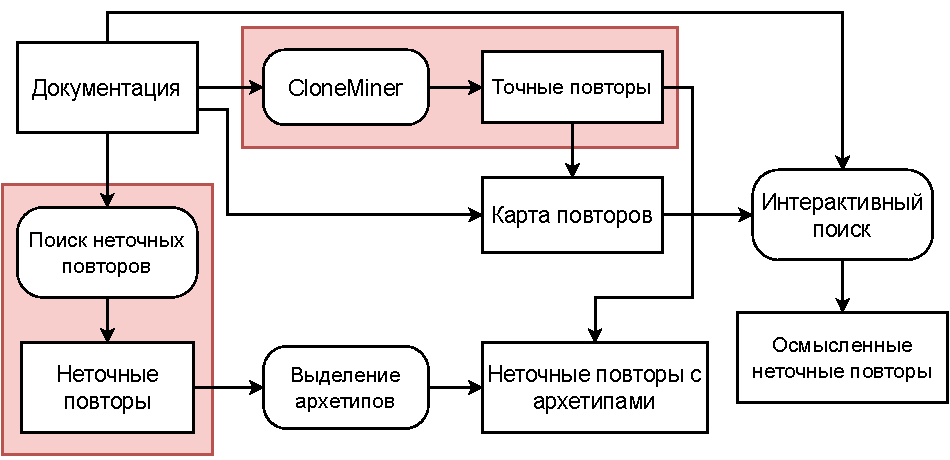
\includegraphics[scale=0.95]{pictures/DuplicateFinder.pdf}
	\centering
	\caption{Схема работы Duplicate Finder. Красным отмечены компоненты, которые планируется заменить.}
	\label{fig:DuplicateFinder}
\end{figure}

Сам поиск повторов делится на две категории --- поиск точных и неточных повторов. В Duplicate Finder для этого используются внешние инструменты: CloneMiner \cite{bib:tool:CloneMiner} для точных повторов, FuzzyRepetitions \cite{bib:tool:FuzzySearch} и NgrammSearch \cite{bib:tool:ImprovedNgramSearch} для неточных. Механизм выглядит следующим образом: на этапе поиска повторов нужный инструмент вызывается при помощи CLI, потом результаты его работы читаются из файла, конвертируются в общий формат, и затем происходит переход на следующий этап. Далее рассмотрим недостатки такого подхода.

Основной проблемой является неоднородность компонентов для поиска. Во-первых --- они написаны на разных языках --- Python, C++, C\#, что влечет за собой необходимость в дополнительных внешних зависимостях и эмуляторах для поддержки кроссплатформенности. Во-вторых --- они абсолютно изолированы друг от друга, что мешает унификации поиска повторов. Несмотря на то, что некоторые шаги можно объединить: загрузка и обработка документа, передача параметров, запись результатов, каждый инструмент повторяет весь процесс поиска с нуля.

Кроме того, каждый инструмент является отдельным проектом, в связи с чем возникает проблема поддержки ---  у каждого инструмента свои авторы и свой жизненный цикл. На данный момент ни один из них больше не разрабатывается и не поддерживается. Особенно острой проблемой это является для CloneMiner. Это единственный инструмент для поиска точных повторов и от него зависит много функционала Duplicate Finder, однако он является закрытой разработкой и от него есть только готовый бинарный файл для Windows, что, сильно мешает развитию проекта в целом. 

Проблемой также является ограниченность интерфейсов этих инструментов. Каждый из них предоставляет возможность передавать набор параметров, однако их разнообразие достаточно ограниченно. Кроме того, все интерфейсы отличаются между собой и даже одни и те же настройки передаются по-разному, что вносит дополнительные неудобства в работу. Также у каждого инструмента свой формат результатов, из-за чего требуется достаточно много дополнительной обработки для преобразования групп повторов во внутреннее представление Duplicate Finder, что затрудняет расширение проекта.

В таблице \ref{table:SearchTools} приведена краткая сводка об основных инструментах для поиска повторов в Duplicate Finder.

\begin{table}[h!]
	\centering
	\begin{minipage}{0.9\textwidth}
\begin{adjustbox}{center}
\begin{tabular}{|c|c|c|c|}
	\hline
	Название & Тип повторов & Язык & Тип лицензии \\
	\hline
	\hline
	CloneMiner & Точные & С++ & Закрытая \\
	\hline
	FuzzyRepetitions & Неточные & C\# & Открытая \\
	\hline
	NgrammSearch & Неточные & Python & Открытая \\
	\hline
\end{tabular}
\end{adjustbox}
\end{minipage}

	\caption{Инструменты поиска повторов.}
	\label{table:SearchTools}
\end{table}

\subsection{Определение требований}
Новый механизм поиска призван устранить обозначенные выше проблемы. Для его разработки необходимо определить основные требования, выполнение которых позволить добиться этой цели. Для нового инструмента поиска повторов были сформулированы следующие функциональные и нефункциональные требования.

\begin{enumerate}
	\item Инструмент должен быть написан на языке Python для максимальной совместимости c Duplicate Finder.
	\item Инструмент должен быть открытой разработкой.
	\item Должна существовать возможность поиска как точных так и неточных повторов, при этом должен быть единый интерфейс.
	\item Процесс поиска должен быть универсальным и различаться только в основном применяемом алгоритме.
	\item Инструмент должен иметь как API для использования в качестве библиотеки, так и CLI для внешнего использования.
	\item Должен предоставляться обширный набор параметров для настройки поиска.
\end{enumerate}

%==============================================================================
\section{Проектирование механизма поиска}
В данной главе подробно описываются логика построения основного конвеера механизма поиска, его этапы, а также алгоритмы для поиска точных и неточных повторов.

\subsection{Схема конвейера}

Кроме непосредственно алгоритмов поиска повторов, процесс поиска в целом может содержать различные вспомогательные шаги. Эти шаги предназначены для улучшения работы алгоритмов и качества результатов, и могут применяться в независимости от конкретного алгоритма. Данная идея лежит в основе разработанного конвейера для механизма поиска. Таким образом, процесс работы будет максимально унифицирован, а компоненты, на которые он разделен, будут обладать низкой связностью. На схеме, представленной на рисунке \ref{fig:Pipeline}, изображены основные этапы конвейера. Далее рассмотрим каждый из них подробно.

\begin{figure}[h!]
	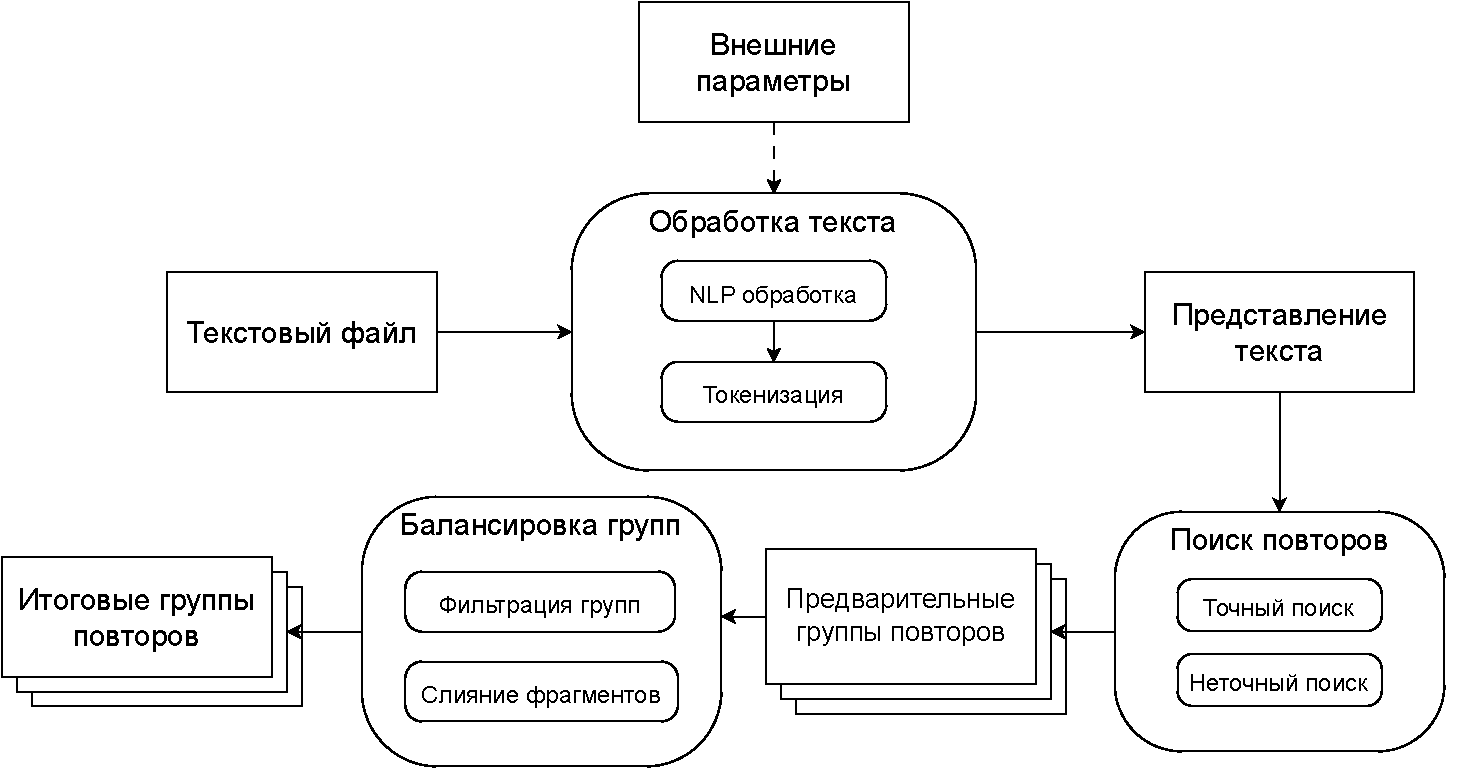
\includegraphics[scale=0.62]{pictures/Pipeline.pdf}
	\centering
	\caption{Схема конвейера механизма поиска.}
	\label{fig:Pipeline}
\end{figure}

\subsection{Предобработка текста}

Сперва стоит обратить внимание на то, что основной целью механизма будет поиск повторов в документации. Документация может быть описательной или справочной, однако в обоих случаях она обычно представляет собой комбинацию текста на естественном языке и исходного кода, хоть и в различных пропорциях. Из-за этой особенности по сути ее можно воспринимать как простой текст, так как в ней отсутствует строгая структура программы. Это значит, что главным фокусом будет нахождение текстовых повторов.

При проектировании механизма в первую очередь нужно подумать про то, какие шаги приведут к наиболее оптимальному результату поиска. Так как найденные фрагменты в конечном итоге нужны пользователю для улучшения документации, чем более семантически осмысленными они будут --- тем лучше. Это, означает, что для улучшения результатов необходимо сначала каким-то образом обработать текст. В данной ситуации хорошо подойдут методы NLP \cite{bib:art:NLP}, часто используемые в машинном обучении \cite{bib:art:Preprocessing}, например, в нейронный сетях \cite{bib:art:NeuralNetworks, bib:tool:NeuroDupDetect}, для работы с естественными языками. Далее перечислим основные подходы, которые можно применить при предобработке текста в механизме поиска.

\textbf{Фильтрация спецсимволов}. Тексты часто содержат большое количество специальных символов. Для естественного языка они в основном представлены пунктуацией, для исходного кода --- различные управляющие символы языка, такие как скобки и кавычки. Хотя такие символы и могут иметь некоторый семантический смысл, они выполняют вспомогательную роль и плохо отражают содержание. Кроме того, они сильно мешать поиску повторов, так как вносят значительные помехи. Поэтому первым шагом необходимо очистить текст от всех спецсимволов.

\textbf{Удаление стоп слов}. В естественных языках присутствует множество вспомогательных слов --- предлоги, частицы, артикли и т.п., которые также не относятся к содержанию. Они называются стоп слова. Такие слова часто встречаются в тексте и распределены достаточно равномерно, из-за чего они по сути являются шумом, поэтому удаление стоп слов при обработке текста является часто применяемой практикой в машинном обучении. Данный подход будет использоваться в качестве второго шага обработки.

Для поиска точных повторов предобработка включает только два шага, обозначенные выше, так как следующие шаги подразумевают трансформацию слов. Это позволяет улучшить поиск неточных повторов, однако в такой ситуации теряется смысл точного поиска.

\textbf{Лемматизация}. Так как нашей целью является поиск содержательных повторов, хорошей идеей будет избавиться от различных грамматических особенностей естественных языков. Это особенно хорошо применимо к документации, учитывая, что в исходном коде также нередко встречаются разнообразные обычные слова (названия переменных, функций, комментарии и т.п.). В этом может помочь такой процесс как лемматизация --- приведение слова к его нормальной форме. В результате применения этого подхода в тексте будет больше одинаковых слов, что увеличит качество находимых повторов.

\textbf{Стемминг}. Еще один подход, который по большей части выполняет ту же самую роль, что и лемматизация --- это стемминг. Данный процесс представляет собой выделение из слова его основу, что позволяет игнорировать грамматические особенности языка. Как и лемматизация, способствует более хорошему поиску повторов.

Также очень важную роль играет способ представления обработанного текста, так как от этого зависит, какие методы можно будет использовать. Практически везде текст разбивается на токены, которые потом используются в качестве минимальной единицы обработки. Однако, в разных инструментах используются различные структуры для представления текста. Самые распространенные --- это дерево токенов и массив токенов. Первый вариант обычно используется при работе со структурированными документами, такими как исходный код, второй --- при работе с естественными текстами, что больше подходит к нашей задаче. Таким образом, результатом этапа предобработки текста будет являться представление текста в виде массива токенов.

Помимо этого, токены разбиваются на классы эквивалентности, и каждому классу присваивается свое число-идентификатор. Это позволяет представлять токены в виде чисел, что облегчает дальнейшую обработки и дает возможность легко их сравнивать: если у двух токенов равны эти идентификаторы, то считается, что соответствующие им участки исходного текста также одинаковы. Кроме того, благодаря такому подходу можно влиять на процесс предобработки извне, указывая какие токены будут считаться эквивалентными.

\subsection{Поиск точных повторов}

Поиск точных повторов подразумевает нахождение фрагментов текста, которые абсолютно идентичны друг другу. В Duplicate Finder для этого использовался CloneMiner \cite{bib:tool:CloneMiner} --- инструмент для поиска клонов в ПО. Особенностью данного инструмента является подход, основанный на последовательности токенов: в отличие от многих других средств, которые используют синтаксическое дерево программы \cite{bib:tool:ASTSearch}, CloneMiner работает с программой как с простым текстом, поэтому его можно применять вне области его предназначения.

Идею алгоритма для поиска точных повторов можно позаимствовать у CloneMiner. Хотя в работе \cite{bib:tool:CloneMiner} отсутствует полноценное описание алгоритма, лежащего в основе инструмента, а его реализация является закрытым проектом, авторы упоминают основные применяемые подходы. В частности, для поиска повторов вместо часто используемого суффиксного дерева \cite{bib:art:SuffixTree} используется суффиксный массив \cite{bib:art:SuffixArray}. Так как документация представляет собой простой текст, такой подход хорошо подойдет для нашей задачи. Изначально использование суффиксного массива подразумевает работу со строками, однако несложно обобщить работу с ним для токенов. Так как в качестве повторов нас интересуют фрагменты текста, будем рассматривать весь документ как строку, а каждый токен как ее символ. Тогда, построив суффиксный массив, можно будет сразу находить целые фрагменты текста, являющиеся точными повторами.

Суффиксный массив представляет собой последовательность индексов суффиксов строки, упорядоченных в лексиграфическом порядке. Можно заметить, что в таком случае суффиксы, начинающиеся с одинаковых подстрок, будут находиться рядом в суффиксном массиве. Так как массив содержит все суффиксы строки, таким образом можно найти все точные повторы в тексте, кроме того, они будут сразу сгруппированы. Для упрощения сравнения рядом стоящих суффиксов можно использовать вспомогательную структуру --- LCP\footnote{Longest Common Prefix --- массив наибольших общих префиксов} массив \cite{bib:art:LCPArray}, которой содержит информацию о том, какая часть соседних суффиксов совпадает. Примеры этих двух структур приведены на рис. \ref{fig:SA-LCP}

\begin{figure}[h!]
	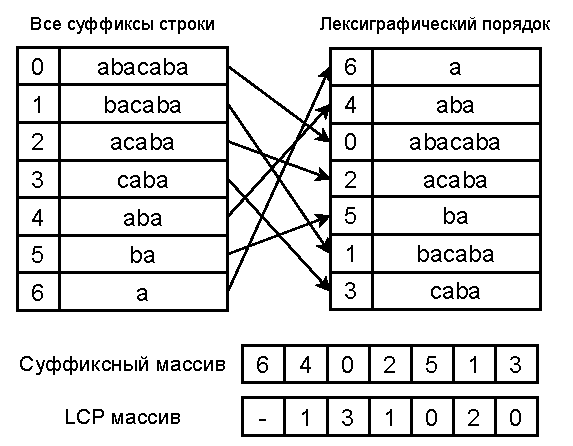
\includegraphics[scale=1.25]{pictures/SA-LCP.pdf}
	\centering
	\caption{Пример суффиксного и LCP массивов.}
	\label{fig:SA-LCP}
\end{figure}

\textbf{Описание алгоритма}

Пусть документ представлен в виде последовательности токенов $D = [t_0,...,t_{n-1}]$. Построим для него суффиксный массив $SA = [s_0,...,s_{n-1}]$. Для этого можно воспользоваться Skew-алгоритмом \cite{bib:art:SkewAlg}, который позволяет построить суффиксный массив за $O(n)$ используя поразрядную сортировку (Radix sort). Такой подход хорошо подходит для нашей цели, так как минимальной единицей обработки является токен, если быть точнее --- его id, и используемый алфавит будет достаточно маленького размера. Затем построим LCP массив $L = [l_0,...,l_{n-1}]$ на основе суффиксного, что можно также сделать за $O(n)$ используя идею, описанную в \cite{bib:art:LCPArray}.

После этого будем итерироваться по суффиксному массиву. Определим параметр $m$ как минимальный размер дубликатов. Для каждого суффикса $s_i, i \in [1,n-1]$ значение $l_i$ показывает сколько общих токенов он имеет с $s_{i-1}$, и пока $l_i \ge m$ все эти фрагменты являются повторами одной группы. Когда определены все суффиксы текущей группы $[s_j,...,s_k]$, нужно проверить, являются ли суффиксами других более длинных суффиксов. Для этого каждый суффикс расширяется пока они имеют одинаковый токен слева $t_{s_j - 1} = ... = t_{s_k - 1}$. В конце алгоритма из суффиксов вырезается совпадающий префикс и создается группа точных повторов, а соответствующие токены помечаются как использованные, и далее пропускаются. Таким образом, каждый токен может быть обработан максимум один раз, из-за чего сложность алгоритма будет $O(n)$ от количества токенов, хотя и с достаточно большой константой.


\subsection{Поиск неточных повторов}

Понятие неточных повторов можно определить различными способами. В рамках данной работы, учитывая используемые алгоритмы поиска, под группой неточных повторов будем понимать набор текстовых фрагментов $G = (g_1,...,g_n)$ такой, что для каждой пары $g_i, g_j \in G$ и некоторой функции схожести $f_{sim}$ выполняется неравенство $f_{sim}(g_i, g_j) \le T$, где $T\ge0$ --- заранее определенный параметр. Таким образом, какие фрагменты будут считаться повторами в основном зависит от выбора функции, а строгость отбора --- от параметра.

\subsubsection{Алгоритм на основе редакционного расстояния}

Одним из распространенных способов сравнения строк является редакционное расстояние или расстояние Левинштайна --- минимальное количество операций удаления, вставки и замены символов, которое необходимо для трансформирования одной строки в другую (рис. \ref{fig:Edit-dist}). Этот подход лежит в основе инструмента \cite{bib:tool:FuzzySearch}. Далее рассмотрим алгоритм подробнее.

\begin{figure}[h!]
	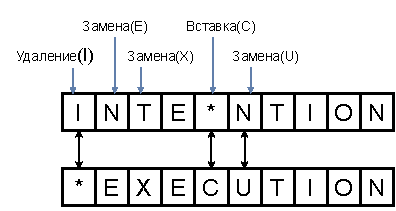
\includegraphics[scale=1.45]{pictures/Edit-dist.pdf}
	\centering
	\caption{Расстояние Левинштайна.}
	\label{fig:Edit-dist}
\end{figure}

Сначала весь текст, представляющий собой последовательность токенов, равномерно разбивается на фрагменты одинакового размера. Затем все фрагменты попарно сравниваются, и если два каких-либо фрагмента достаточно похожи --- они сохраняются как пара повторов. Основной функцией схожести как раз и является редакционное расстояние, исчисляемое как разница в токенах между фрагментами. Так как вычисление редакционного расстояния процесс достаточно трудоемкий, для оптимизации фрагменты сначала сравниваются по их хешам, которые рассчитываются заранее для каждого фрагмента.  Эта оценка является достаточно грубой, но помогает отсеять сильно отличающиеся пары. Граничные значения схожести являются внешними параметрами алгоритма. На последнем этапе пары повторов объединяются в группы и затем проводится расширение повторов в этих групп за счет объединения с соседними фрагментами и удаления пересечений между группами.

Хотя основную концепцию данного подхода можно оставить, у оригинального инструмента есть ряд недостатков, решив которые можно улучшить алгоритм поиска:
\begin{itemize}
	\item могут обрабатываться только документы в формате XML, что сильно сужает область применения;
	\item группы составляются простым перебором пар, что неэффективно и предоставляет мало возможностей для дальнейшей обработки;
	\item используемый подход хеширования достаточно ограничен и дает слишком неточную оценку.
\end{itemize}

\textbf{Описание алгоритма}

Так как предобработкой текста и балансировкой групп занимаются отдельные компоненты, сосредоточим внимание на основной части алгоритма поиска. Будем рассматривать входной документ $D$ как последовательность из $n$ токенов $D = [t_0,...,t_{n-1}]$. Определим размер фрагментов $0 < m < n$ и равномерно разобьем текст на $k = n / m$ фрагментов этого размера (если $n mod m \ne 0$, тогда дополним текст с конца пустыми токенами). В результате получим набор фрагментов $[g_0,...g_{k-1}]$, где $g_i = [t_{i * m},...,t_{i * (m + 1) - 1}]$. 

После разбиения для каждого фрагмента вычислим его отпечаток в виде 32-битного хеша, используя подход sim-hash \cite{bib:art:SimHash}. Для этого посчитаем хеш каждого токена при помощи алгоритма MD5 \cite{bib:art:MD5}. Выбор алгоритма хеширования обусловлен тем, что для наших целей криптографическая стойкость роли не играет, а при этом MD5 вычисляется быстрее популярной альтернативы SHA256 \cite{bib:art:MD5vsSHA256}. Далее для фрагмента $g_i$ определим результирующих хеш $h_i$ на основе хешей токенов: возьмем последние 32 бита каждого из них, и для каждой позиции, если более половины битов равны одному, то в результат запишем 1, иначе 0. Укороченный пример хеширования приведен на рис. \ref{fig:Hashing}.

\begin{figure}[h!]
	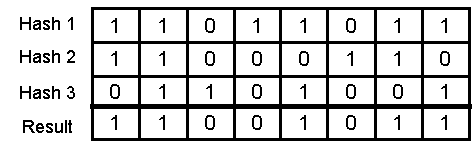
\includegraphics[scale=1.5]{pictures/Hash.pdf}
	\centering
	\caption{Пример вычисления итогового хеша.}
	\label{fig:Hashing}
\end{figure}

Затем происходит попарное сравнение. Если разница в хешах фрагментов $g_i, g_j$, определенная как количество единиц в числе $h_i \oplus h_j$, не превышает определенной границы, то вычисляется редакционное расстояние между фрагментами. Для этого применяется алгоритм Укконена \cite{bib:art:UkkonenASM} для приблизительного сравнения строк (approximate string matching). Данный подход позволяет оптимально дать ответ на вопрос: больше ли редакционное расстояние между элементами, чем заданная граница, что мы и хотим выяснить. Так как размеры фрагментов одинаковы, а максимальное количество допустимых операций константно, сложность вычисления будет $O(m)$. Если в итоге фрагменты успешно проходят оба этапа сравнения, то они записываются, как пара повторов. В общей сложности этот этап замет не больше $O(k^2 * m) = O(\frac{n^2}{m})$

После нахождения всех пар повторов, необходимо объединить их в группы. Можно заметить, что по сути эти пары образуют неориентированный граф, где вершинами являются фрагменты, а ребра отображают их сходство. Графы очень широко распространены и имеют множество применений в разных областях, и, соответственно, существует большое количество различных алгоритмов и подходов для работы с графами, поэтому такое представление является очень выгодным. Составление групп повторов происходит путем поиска компонент связности полученного графа. Как более строгий, но медленный вариант можно использовать, например, поиск всех клик\footnote{Клика --- максимальный полный подграф} графа. Так как поиск компонент связности даже в худшем случае не будет превышать $O(c^2)$, в целом сложность алгоритма можно оценить как $O(\frac{n^2}{m})$ от количества токенов и размера фрагментов.

\subsubsection{Алгоритм на основе N-грамм}

Еще один распространенный подход при работе с текстами --- это N-граммы \cite{bib:art:Ngram}. Построив множества N-грамм для двух фрагментов, можно затем получить оценку их схожести на основе сравнения этих множеств. На рисунке \ref{fig:Ngram} приведен пример таких множеств для различных N. На этом принципе основан алгоритм поиска, описанный в статье \cite{bib:tool:NgramSearch}. Улучшенная версия данного алгоритма приводится в работе \cite{bib:tool:ImprovedNgramSearch}.

\begin{figure}[h!]
	\includegraphics[scale=0.37]{pictures/Ngram.png}
	\centering
	\caption{Пример множеств N-грам \cite{bib:fig:Ngram}.}
	\label{fig:Ngram}
\end{figure}

Отдельно рассматривать этот алгоритма смысла нет, так как описанная ниже итоговая версия по большей части совпадает с ним, однако стоит отметить некоторые недостатки, которые можно устранить для дальнейшего его улучшения:

\begin{itemize}
	\item алгоритм содержит большое количество последовательных пересечений с множествами одних и тех же фрагментов, однако так как пересечение множеств --- операция ассоциативная, достаточно вычислить пересечение группы один раз;
	\item в работе описывается только работа с 3-граммами, однако алгоритм можно обобщить для любых N.
\end{itemize}

\textbf{Описание алгоритма}

Разобьем входной документ на набор предложений:	$D = [s_0,\dots,s_{n-1}]$. Для каждого предложения $s_i$ вычислим множество N-грам $N_i$. Изначально определим каждое предложение в отдельную группу повторов $G_i$, и для каждой такой группы будем поддерживать множество N-грам, которое будет являться пересечением таких множеств каждого предложения этой группы $N_{G_i} = \cap N_j, N_j\in G_i$. Затем будем пытаться добавить каждое предложение к какой-либо группе: для $s_i$ и группы $G_k, k\in[0\dots i-1, i+1\dots n-1]$ вычислим мощность пересечения его множества N-грам с множеством группы-кандидата $overlap_k = |N_i \cap N_{G_k}|$. Затем выберем группу с максимальным пересечением $j = \argmax\limits_{k} (overlap_k)$ и если $overlap_j > T$, где $T$ - заранее заданная граница, то добавляем предложение $s_i$ к группе $G_j$, обновляя $N_{G_j} = N_{G_j} \cap N_i$. После итерации по всем предложениям, результатом работы алгоритма будет набор групп неточных повторов.

Рассмотрим сложность алгоритма. Так как количество предложений линейно зависит от общего количества токенов, дальнейшие расчеты будем проводить относительно предложений. Также стоит отметить, что предложение состоит из константного количества токенов, как, соответственно и множество его N-грам. Пересечение двух множеств можно вычислить за $O(\min(k_i, k_j))$, где $k_i, k_j$ - размеры множеств. Итерация по всем предложениям займет $O(n)$, для каждого предложения нужно пересечь его множества с каждой группой. Само пересечение в нашей ситуации выполняется за $O(1)$. В худшем случае, если в тексте нет повторов, то количество групп будет всегда равно $n$. На практике, хоть количество групп и будет уменьшаться, повторы покрывают не очень большую часть текста. Таким образом, сложность алгоритма можно оценить как $O(n^2)$ от количества токенов.

\newpage
\subsection{Балансировка групп повторов}

Результатом работы алгоритмов поиска является набор групп повторов. Так как основная задача инструмента --- это поиск простых текстовых повторов, дальнейшие анализ или обработка полученных групп фрагментов с точки зрения семантики не требуется. Однако можно попробовать улучшить эти группы: во-первых --- избавиться от возможных нежелательных последствий, которые могут возникнуть в результате работы алгоритма, а во-вторых --- попробовать, манипулируя фрагментами, изменить сами группы, чтобы увеличить их осмысленность. Далее подробно рассмотрим конкретные шаги, которые позволят добиться оптимального разбиения фрагментов на группы.

\textbf{Фильтрация}

Первым и последним шагом этого процесса является фильтрация незначимых групп. В результате работы некоторых алгоритмов, среди групп повторов могут быть пустые или содержащие только один фрагмент. Такие группы не представляют никакого интереса и их нельзя использовать для дальнейшей обработки, поэтому их стоит просто удалить. Особенно много таких групп может возникнуть в результате работы следующего шага из-за перестановок фрагментов между группами.

\textbf{Балансировка}

В зависимости от особенностей исходного текста и алгоритма поиска, повторы могут быть объединены в группы не лучшим образом. Для оценки качества разбиения нужно ввести некоторую метрику. Рассмотрим основные параметры, которые влияют на качество группы повторов:

\begin{itemize}
	\item количество повторов в группе --- чем больше какой-либо фрагмент повторяется в тексте, тем больше интереса он представляет;
	\item длина повторов в группе --- чем длиннее найденные фрагменты, тем больше шанс, что они будут содержать более осмысленную информацию.
\end{itemize}

На основе этих параметров можно ввести простую функцию значимости группы:
\begin{equation}
	f_{sig} = n * m^2
\end{equation}
где n - количество повторов, m - средняя длина.

Рассмотрим две группы повторов, а точнее как расположены их фрагменты в тексте. В общем случае может быть 3 варианта их взаимного расположения.
\begin{enumerate}
	\item Фрагменты двух групп не находятся рядом (рис. \ref{fig:Balance1}). В таком случае ничего сделать не получится.
	\item Некоторые фрагменты двух групп являются соседями в тексте (рис. \ref{fig:Balance2}). Теоретически соседние фрагменты можно объединить в один более длинный. Однако, так как группы пересекаются лишь частично, нельзя гарантировать, что такое объединение не нарушит логической целостности групп. Таким образом, в этом случае также не стоит изменять группы.
	\item Все фрагменты одной группы находятся рядом с фрагментами другой. В таком случае можно попробовать объединить эти фрагменты, удалив их из другой группы как показано на рисунке \ref{fig:Balance3}. Для этого воспользуемся функцией значимости: будем проводить эту операцию, если после нее увеличится значимость групп: $f_{sig}(g_i^1) + f_{sig}(g_j^1) < f_{sig}(g_i^2) + f_{sig}(g_j^2)$. Частный случай --- если в группах одинаковые количества повторов, тогда можно их сразу склеить.
\end{enumerate}

\begin{figure}[ht!]
	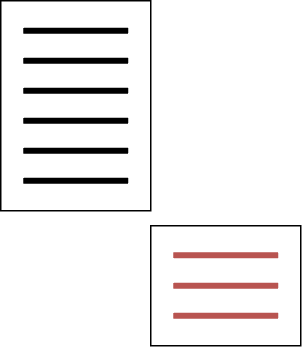
\includegraphics[scale=0.5]{pictures/Balance1.png}
	\centering
	\caption{Группы повторов, не имеющие соседних фрагментов.}
	\label{fig:Balance1}
\end{figure}

\begin{figure}[h!]
	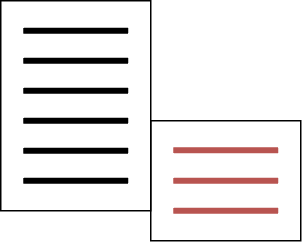
\includegraphics[scale=0.5]{pictures/Balance2.png}
	\centering
	\caption{Группы повторов, содержащие некоторые соседние фрагменты.}
	\label{fig:Balance2}
\end{figure}

\begin{figure}[h!]
	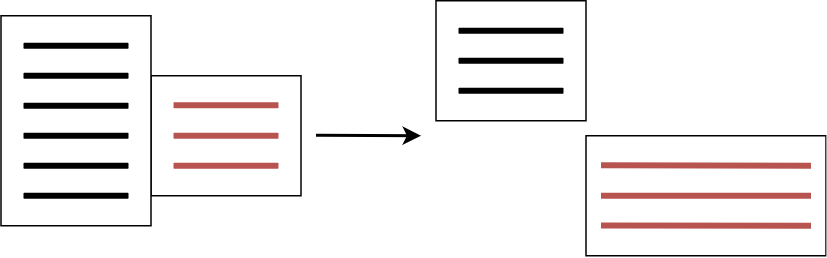
\includegraphics[scale=0.5]{pictures/Balance3.png}
	\centering
	\caption{Все фрагменты одной группы повторов являются соседями фрагментов другой.}
	\label{fig:Balance3}
\end{figure}

%==============================================================================
\clearpage
\section{Особенности реализации}

\subsection{Используемые технологии}

Для реализации был использован язык Python версии 3.8, чтобы добиться максимальной совместимости с DuplicateFinder. Среди множества инструментов для работы с естественным языком, ведущей платформой является NLTK(Natural Language Toolkit), представляющая собой набор библиотек для достижения различных целей. В рамках данный работы для предобработки текста использовались следующие технологии:
\begin{itemize}
	\item различные токенизаторы для разбиения текста --- LineTokenizer, WordPunctTokenizer, SentTokenizer;
	\item реализация алгоритма стемминга --- PorterStemmer;
	\item пакет для лемматизации --- WordNetLemmatizer.
\end{itemize}

Так как Python имеет динамическую типизацию, для облегчения процесса разработки также использовалась технология MyPy, позволяющая использовать подсказки типов в Python'е для статического анализа кода на соответствие типов.

\subsection{Архитектура}

Основной задачей при разработке архитектуры было разбиение этапов конвейера на отдельные компоненты и поддержка низкой связности этих компонент. Такой подход позволит легко добавлять в инструмент новые методы токенизации и алгоритмы поиска. Кроме того, он предоставляет широкие возможности для манипулирования всем процессом поиска: для каждого этапа можно выбирать одну из существующих компонент, подстраивая инструмент под конкретную задачу. Схема архитектуры представлена ниже на рисунке \ref{fig:Architecture}.

\begin{figure}[h!]
	\centering
	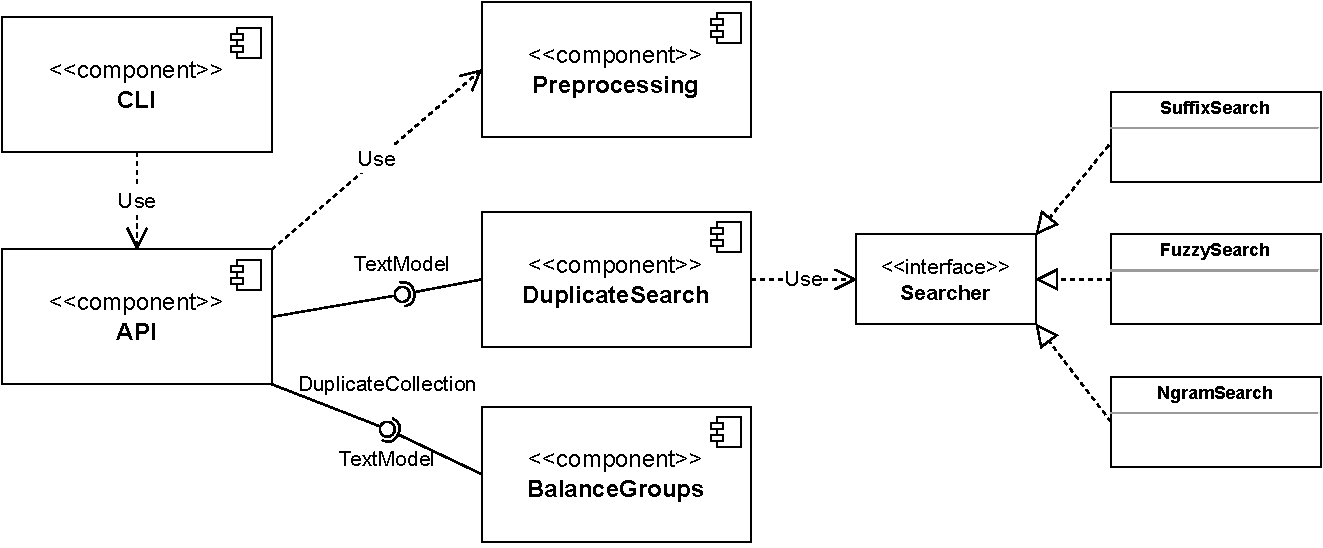
\includegraphics[scale=0.7]{pictures/Architecture.pdf}
	\caption{Архитектура механизма поиска.}
	\label{fig:Architecture}
\end{figure}

Каждому основному этапу конвейера соответствует своя компонента: предобработка, поиск повторов и балансировка полученных групп. Также три реализованных алгоритма поиска представлены отдельными классами, являющимися реализацией единого интерфейса поисковика. Инструмент имеет API и CLI, таким образом его можно использовать и в качестве Python пакета, и в виде независимого скрипта.

%==============================================================================
\clearpage
\section{Тестирование}

Для того, чтобы убедиться в корректности и качестве разработанного инструмента (далее --- TextDuplicateSearch), необходимо провести ряд тестов. Во-первых, нужно проверить то, как находятся точные и неточные повторы, а во-вторых --- как инструмент работает с Duplicate Finder.

Для тестирования были выбраны документации ряда крупных проектов: Blender, GIMP, PostgreSQL, Zend Framework, Apache Subversion. Информация о документах приведена в таблице \ref{table:Documents}. 

\begin{table}[ht!]
	\centering
	\include{tables/Documents.tex}
	\caption{Документы, выбранные для тестирования.}
	\label{table:Documents}
\end{table}

Для этих документов был проведен поиск точных и неточных повторов, и собрана статистика по найденным группам. Характеристиками, представляющими наибольший интерес, являются количество групп повторов и их размер, а также длина фрагментов в токенах. Результаты приведены ниже в таблицах \ref{table:StrictSearch} и \ref{table:FuzzySearch}. Поиск проводился с фильтрацией стоп слов и ограничением на минимальный размер клона $n=10$.

Можно заметить, что, несмотря на небольшую выборку, практические результаты в целом отображают теоретические ожидания: не в зависимости от типа документа или проекта, около 10\% документации крупных проектов является дублированными фрагментами. Исключением являются Python Requests и в некоторой мере PostgreSQL Manual, являющиеся справочной документацией и в основном состоящие из описания методов. Это подтверждает идею о том, что повторы в документации не являются негативной чертой сами по себе, и иногда даже необходимы.

\begin{table}[ht!]
	\centering
	\begin{minipage}{0.9\textwidth}
\begin{adjustbox}{center}
\begin{tabular}{|l||c|c|c|c|}
	\hline
	& GIMP & PostgreSQL & Subversion & Zend Framework \\
	\hline
	\hline
	Токены & 132554 & 72728 & 110270 & 164035 \\
	\hline
	Группы повторов & 400 & 289 & 218  & 557 \\
	\hline
	Средний размер группы & 2.57 & 2.30 & 2.17 & 2.44 \\
	\hline
	Средняя длина повтора & 14.59 & 16.31 & 17.27 & 16.58 \\
	\hline
	Покрытие документа & ~11\% & ~14\% & ~7\% & ~13\% \\
	\hline
	
\end{tabular}
\end{adjustbox}
\end{minipage}
	\caption{Результаты точного поиска.}
	\label{table:StrictSearch}
\end{table}

\begin{table}[ht!]
	\centering
	\begin{minipage}{0.9\textwidth}
\begin{adjustbox}{center}
\begin{tabular}{|l||m{0.15\textwidth}|m{0.15\textwidth}|m{0.15\textwidth}|m{0.2\textwidth}|}
	\hline
	Документ & Группы повторов & Средний размер группы & Средняя длина повтора & Покрытие документа \\
	\hline
	\hline
	GIMP Manual & 574 & 2.65 & 13.64 & 15\% \\
	\hline
	PostgreSQL Manual & 464 & 2.66 & 17.17 & 25\% \\
	\hline
	Subversion book & 282 & 2.27 & 18.93 & 10\% \\
	\hline
	Zend Framework guide & 522 & 2.32 & 22.96 & 16\% \\
	\hline
	Blender Manual & 1393 & 2.48 & 14.22 & 16\% \\
	\hline
	Python Requests & 23 & 2.26 & 20.16 & 28\% \\
	\hline
\end{tabular}
\end{adjustbox}
\end{minipage}
	\caption{Результаты неточного поиска.}
	\label{table:FuzzySearch}
\end{table}

\newpage
Так как для Duplicate Finder самым важным является поиск точных повторов, рассмотрим его подробнее. Основным параметром для точного поиска является минимальная длинна повтора $n$: если размер фрагмента в токенах меньше этого числа, то он отбрасывается, даже если является частью группы повторов. На рисунке \ref{fig:StrictSearch} изображен график с результатами точного поиска для имеющегося набора документов с разными значениями этого параметра (без фильтрации стоп слов). Можно наблюдать, что с увеличением минимальной границы количество повторов, и из-за этого и групп, уменьшается, что также соответствует ожиданиям.

\begin{figure}[ht!]
	\centering
	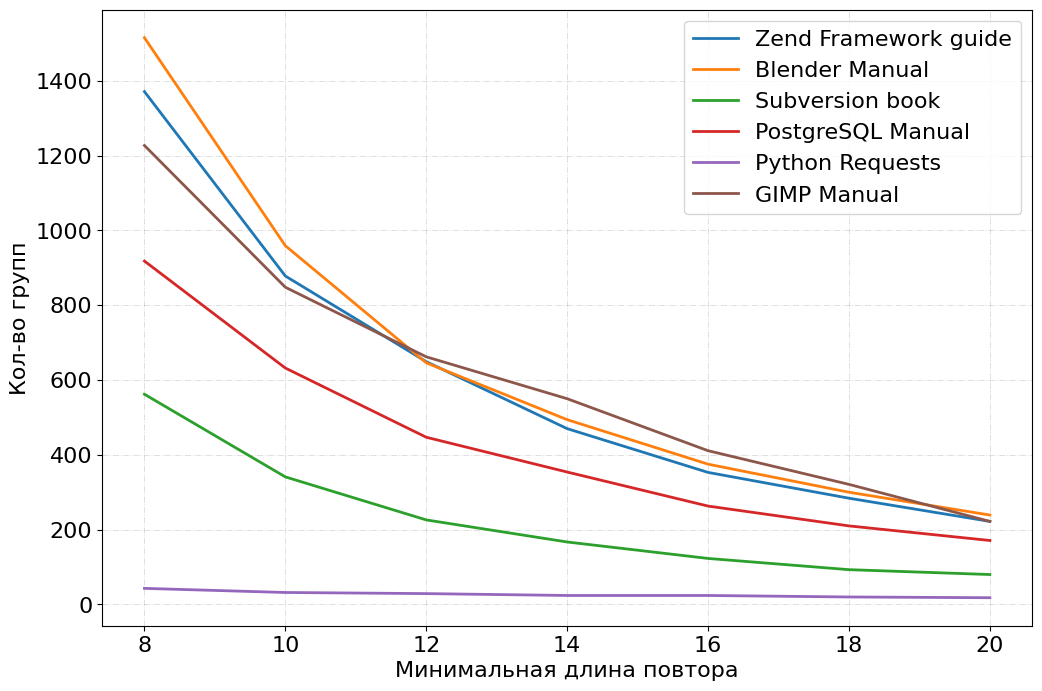
\includegraphics[scale=0.55]{pictures/StrictSearch.png}
	\caption{Результаты точного поиска с переменным параметром.}
	\label{fig:StrictSearch}
\end{figure}

Далее проведем сравнение TextDuplicateSearch с CloneMiner, который использовался в Duplicate Finder. Для каждого документа выполним поиск точных повторов с ограничением $n=20$. Как видно на графике (рис. \ref{fig:Comp1}), оба инструмента находят приблизительно одинаковое количество повторов. Различие состоит в том, каким образом текст разбивается на токены. В общем, CloneMiner преобразует текст в большее количество токенов, из-за чего при одинаковом ограничении $n$ CloneMiner отсеет меньше фрагментов. Однако, это никак не сказывается на качестве: достаточно уменьшить границу для TextDuplicateSearch и эти фрагменты также будут найдены.

\begin{figure}[ht!]
	\centering
	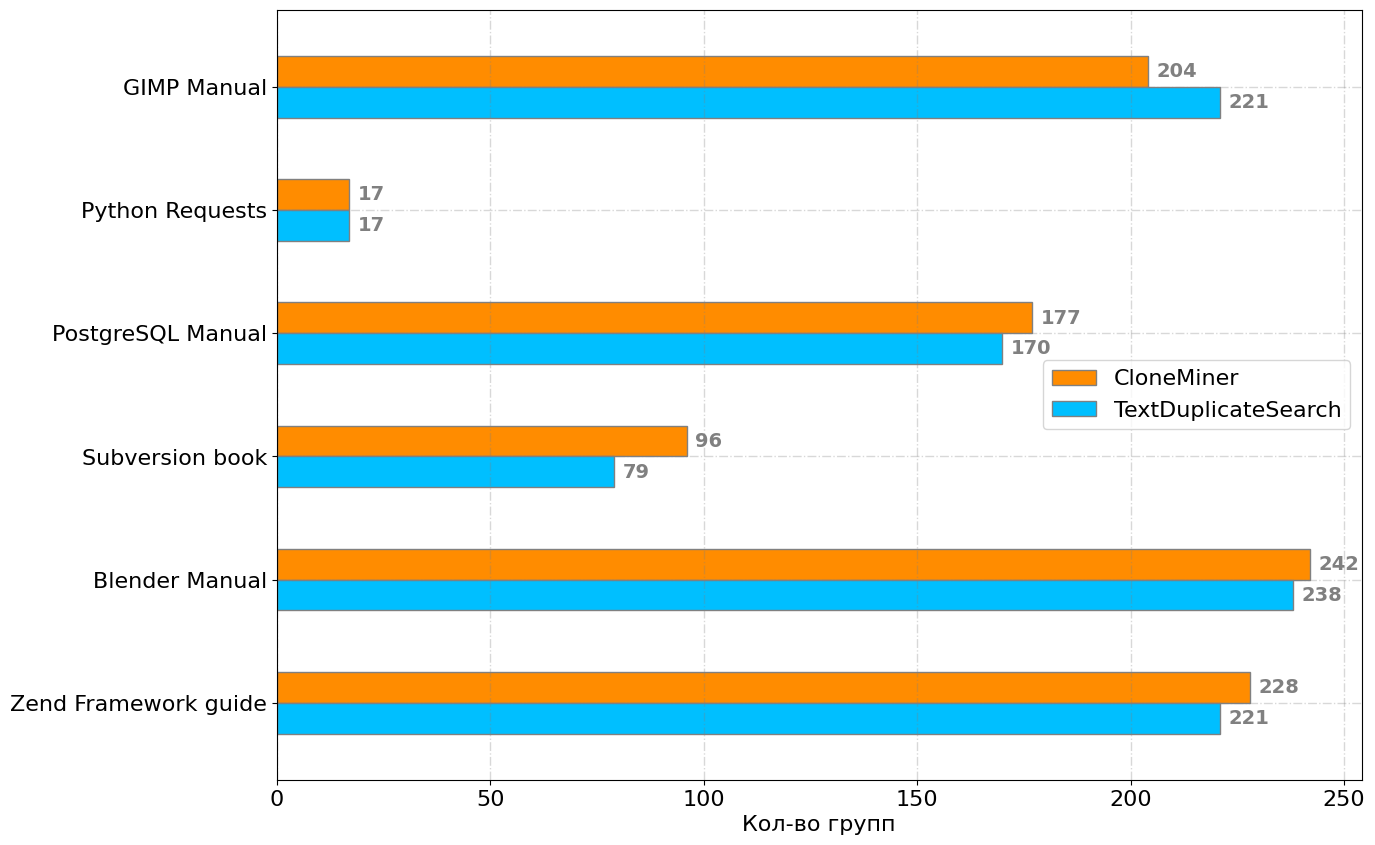
\includegraphics[scale=0.47]{pictures/Comp1.png}
	\caption{Результаты простого поиска.}
	\label{fig:Comp1}
\end{figure}

Затем рассмотрим поиск повторов в рамках Dupicate Finder. Отличие от простого поиска заключается в дополнительной обработке найденных групп, в результате которой получаются осмысленные группы точных и неточных повторов. На графике ниже (рис. \ref{fig:Comp2}) показаны количества итоговых групп, полученные после работы Duplicate Finder. Как можно заметить, после этой обработки в среднем количество групп от CloneMiner сокращается примерно на 31\%, в то время как от TextDuplicateSearch всего на 18\%. Это показывает, что во-первых, реализованный инструмент находит более осмысленные группы, а во-вторых --- то что наличие пересечений между группами CloneMiner, которое отсутствует в TextDuplicateSearch, также негативно сказывается на результатах.

\begin{figure}[h!]
	\centering
	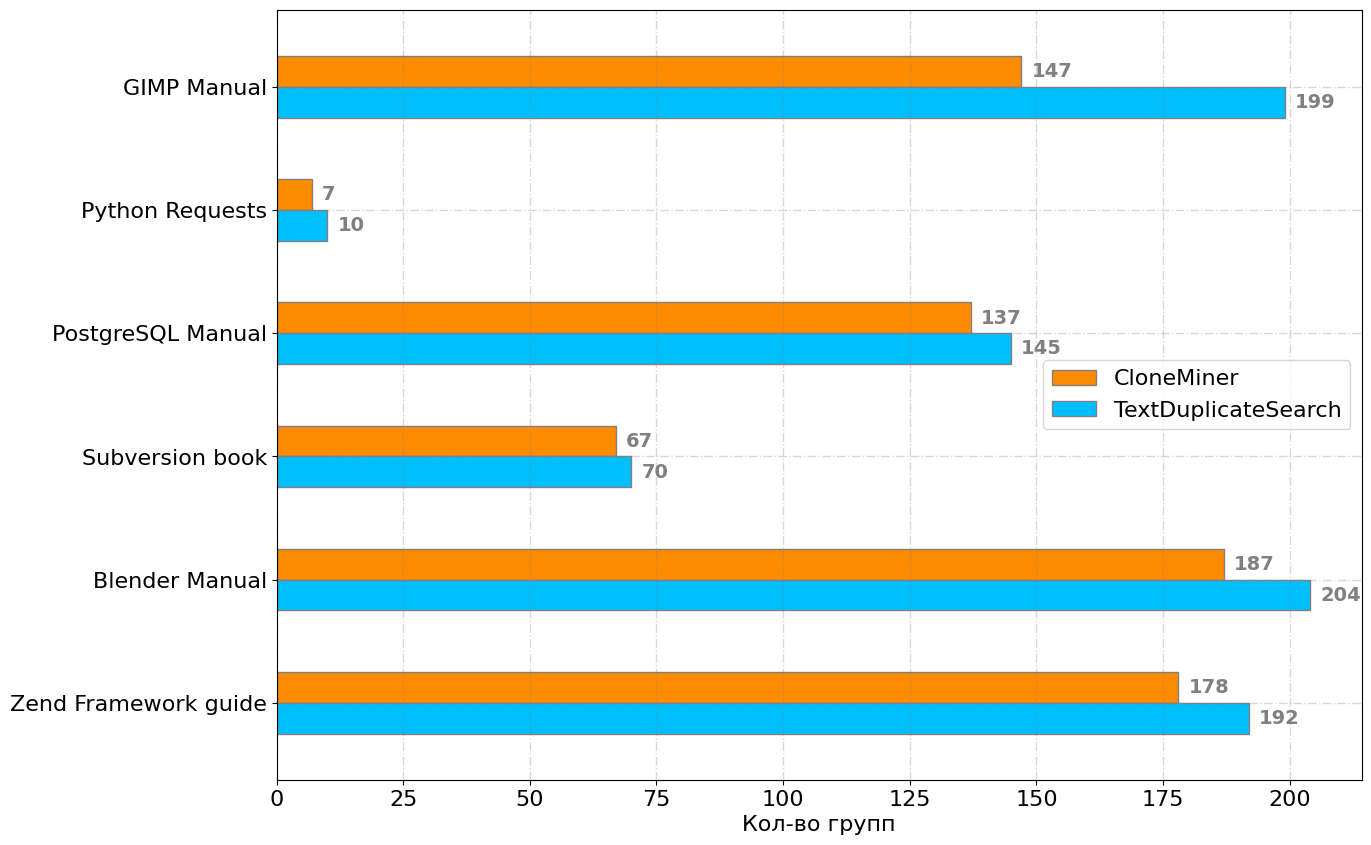
\includegraphics[scale=0.47]{pictures/Comp2.png}
	\caption{Результаты поиска с обработкой Duplicate Finder.}
	\label{fig:Comp2}
\end{figure}

\newpage
Таким образом, по результатам тестирования можно сделать вывод, что реализованный инструмент хорошо находит точные и неточные повторы, при этом в результате поиска получаются более качественные группы по сравнению с инструментами, использованными в Duplicate Finder.

Также стоит взять в расчет производительность. Хотя никаких особых требований в этом плане к работе инструмента нет, поиск все же должен занимать разумное количество времени. Для этого проведем точный поиск повторов для выбранных документов с различными значениями минимального размера повтора $n$. Так как большая точность не нужна, ограничимся размером выборки в 15 запусков для каждого случая. Из-за маленького размера выборки будем рассчитывать 98\%-доверительный интервал на основе распределения Стьюдента.

Для определения времени поиска воспользуемся встроенным в Python профилировщиком cProfile. Замеры производились на машине со следующими характеристиками: Lenovo Legion Y540-15IRH, Windows 10 22H2, Intel\textregistered\ Core\texttrademark\ i5-9300H 2.40GHz, RAM 16 Gb. Результаты приведены в таблице \ref{table:Times}, время указано в секундах.

\begin{table}[ht!]
	\centering
	\begin{minipage}{0.9\textwidth}
\begin{adjustbox}{center}
\begin{tabular}{|l||c|c|c|}
	\hline
	Документ & $n = 10$, c & $n = 15$, c & $n = 20$, c  \\
	\hline
	\hline
	The GIMP user manual  & $10.031\pm0.072$  & $10.102\pm0.075$  & $10.073\pm0.052$ \\
	\hline
	PostgreSQL manual & $4.709\pm0.085$ & $4.652\pm0.070$ & $4.706\pm0.038$ \\
	\hline
	Subversion Book & $7.808\pm0.052$ & $7.77\pm0.064$ & $7.625\pm0.054$ \\
	\hline
	Zend Framework guide & $10.722\pm0.078$ & $10.560\pm0.063$ & $10.536\pm0.073$ \\
	\hline
	Blender Manual & $22.451\pm0.214$ & $22.233\pm0.161$ & $22.130\pm0.215$ \\
	\hline
	Python Requests & $0.116\pm0.007$  & $0.119\pm0.007$ & $0.120\pm0.007$ \\
	\hline
\end{tabular}
\end{adjustbox}
\end{minipage}
	\caption{Время работы точного поиска повторов.}
	\label{table:Times}
\end{table}

Как видно по результатам, время работы инструмента в основном зависит только от размера документа, и практически не зависит от параметра. В целом можно сказать, что поиск производится за приемлемое время.

%==============================================================================
\clearpage
\section*{Заключение}
В ходе данной работы были получены следующие результаты.
\begin{enumerate}
   	\item Проанализированы основные подходы и средства, которые используются в существующих инструментах для поиска повторов: синтаксические и суффиксные деревья, нейронные сети, обработка естественного языка, алгоритмы хеширования, N-граммы.
   	\item Выявлены следующие основные требования к новому механизму поиска: объединение точного и неточного поиска, унификация процесса поиска, высокая степень настраиваемости.
   	\item Спроектирован конвейер для механизма поиска, состоящий из трех основных этапов: предобработка текста, применение алгоритмов поиска повторов, балансировка групп повторов.
   	\item Разработаны алгоритмы для точного и неточного поиска повторов на основе использованных в Duplicate Finder инструментов.
   	\item Выполнена реализация инструмента на языке Python с использованием пакета NLTK для предобработки текста, исходный код выложен на GitHub и доступен по ссылке \url{https://github.com/IceWind2/TextDuplicateSearch}; проведена интеграция с Duplicate Finder.
   	\item Проведено тестирование инструмента на корпусе документов, по результатам работы собрана статистика и проведен ее анализ.
\end{enumerate}

%==============================================================================

\setmonofont[Mapping=tex-text]{CMU Typewriter Text}
\bibliographystyle{ugost2008ls}
\bibliography{diploma}
\end{document}
